\documentclass[../main.tex]{subfiles}

Das Infrarotspektrometer ist ein Werkzeug der Spektroskopie, das mithilfe der Absorptionseigenschaften der Elemente am Infrarotlicht Eigenschaften von Substanzen nachweisen kann. Spezifisch sind es innermolekulare Bindungen, anhand dessen die gemessene Substanz nachgewiesen werden kann. 

\subsection{Komponenten}

\begin{figure}[ht]
    \centering
    \begin{subfigure}[b]{0.25\textwidth}
        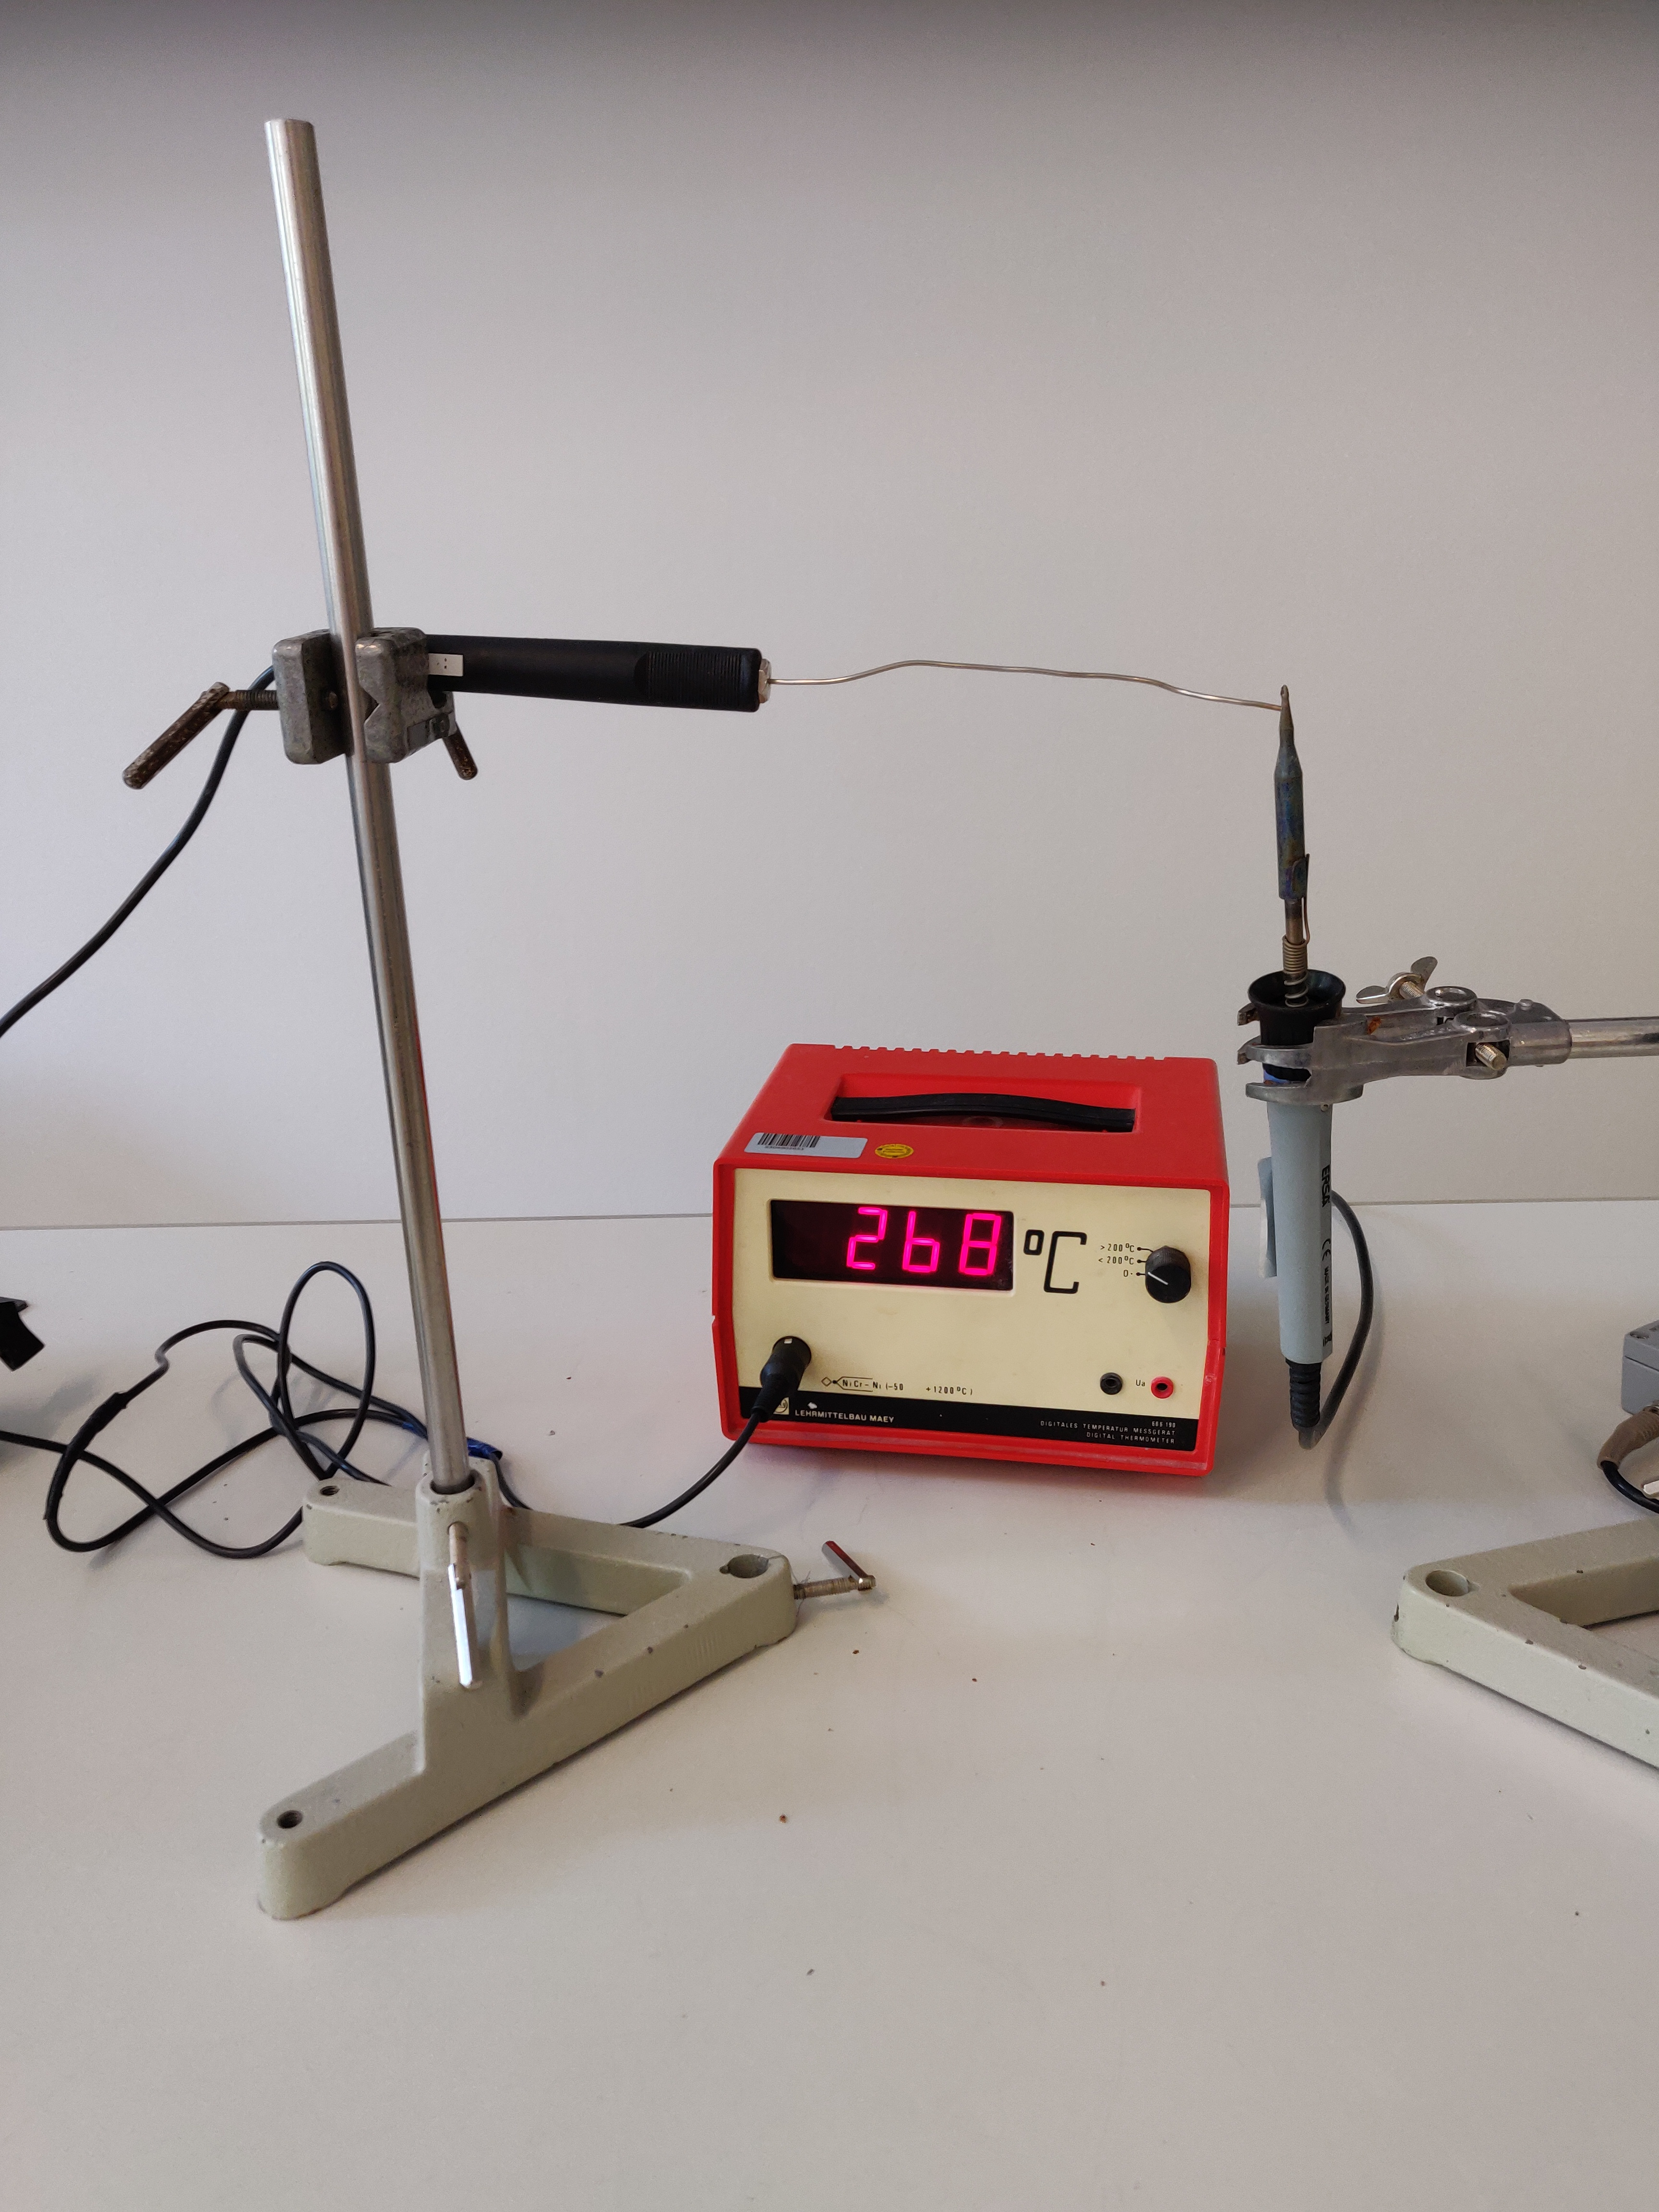
\includegraphics[width=\textwidth]{experiment/11-loetkolben-temperatur.jpg}
        \caption{Lötkolben}
        \label{fig:loetkolben}
    \end{subfigure}
    \begin{subfigure}[b]{0.25\textwidth}
        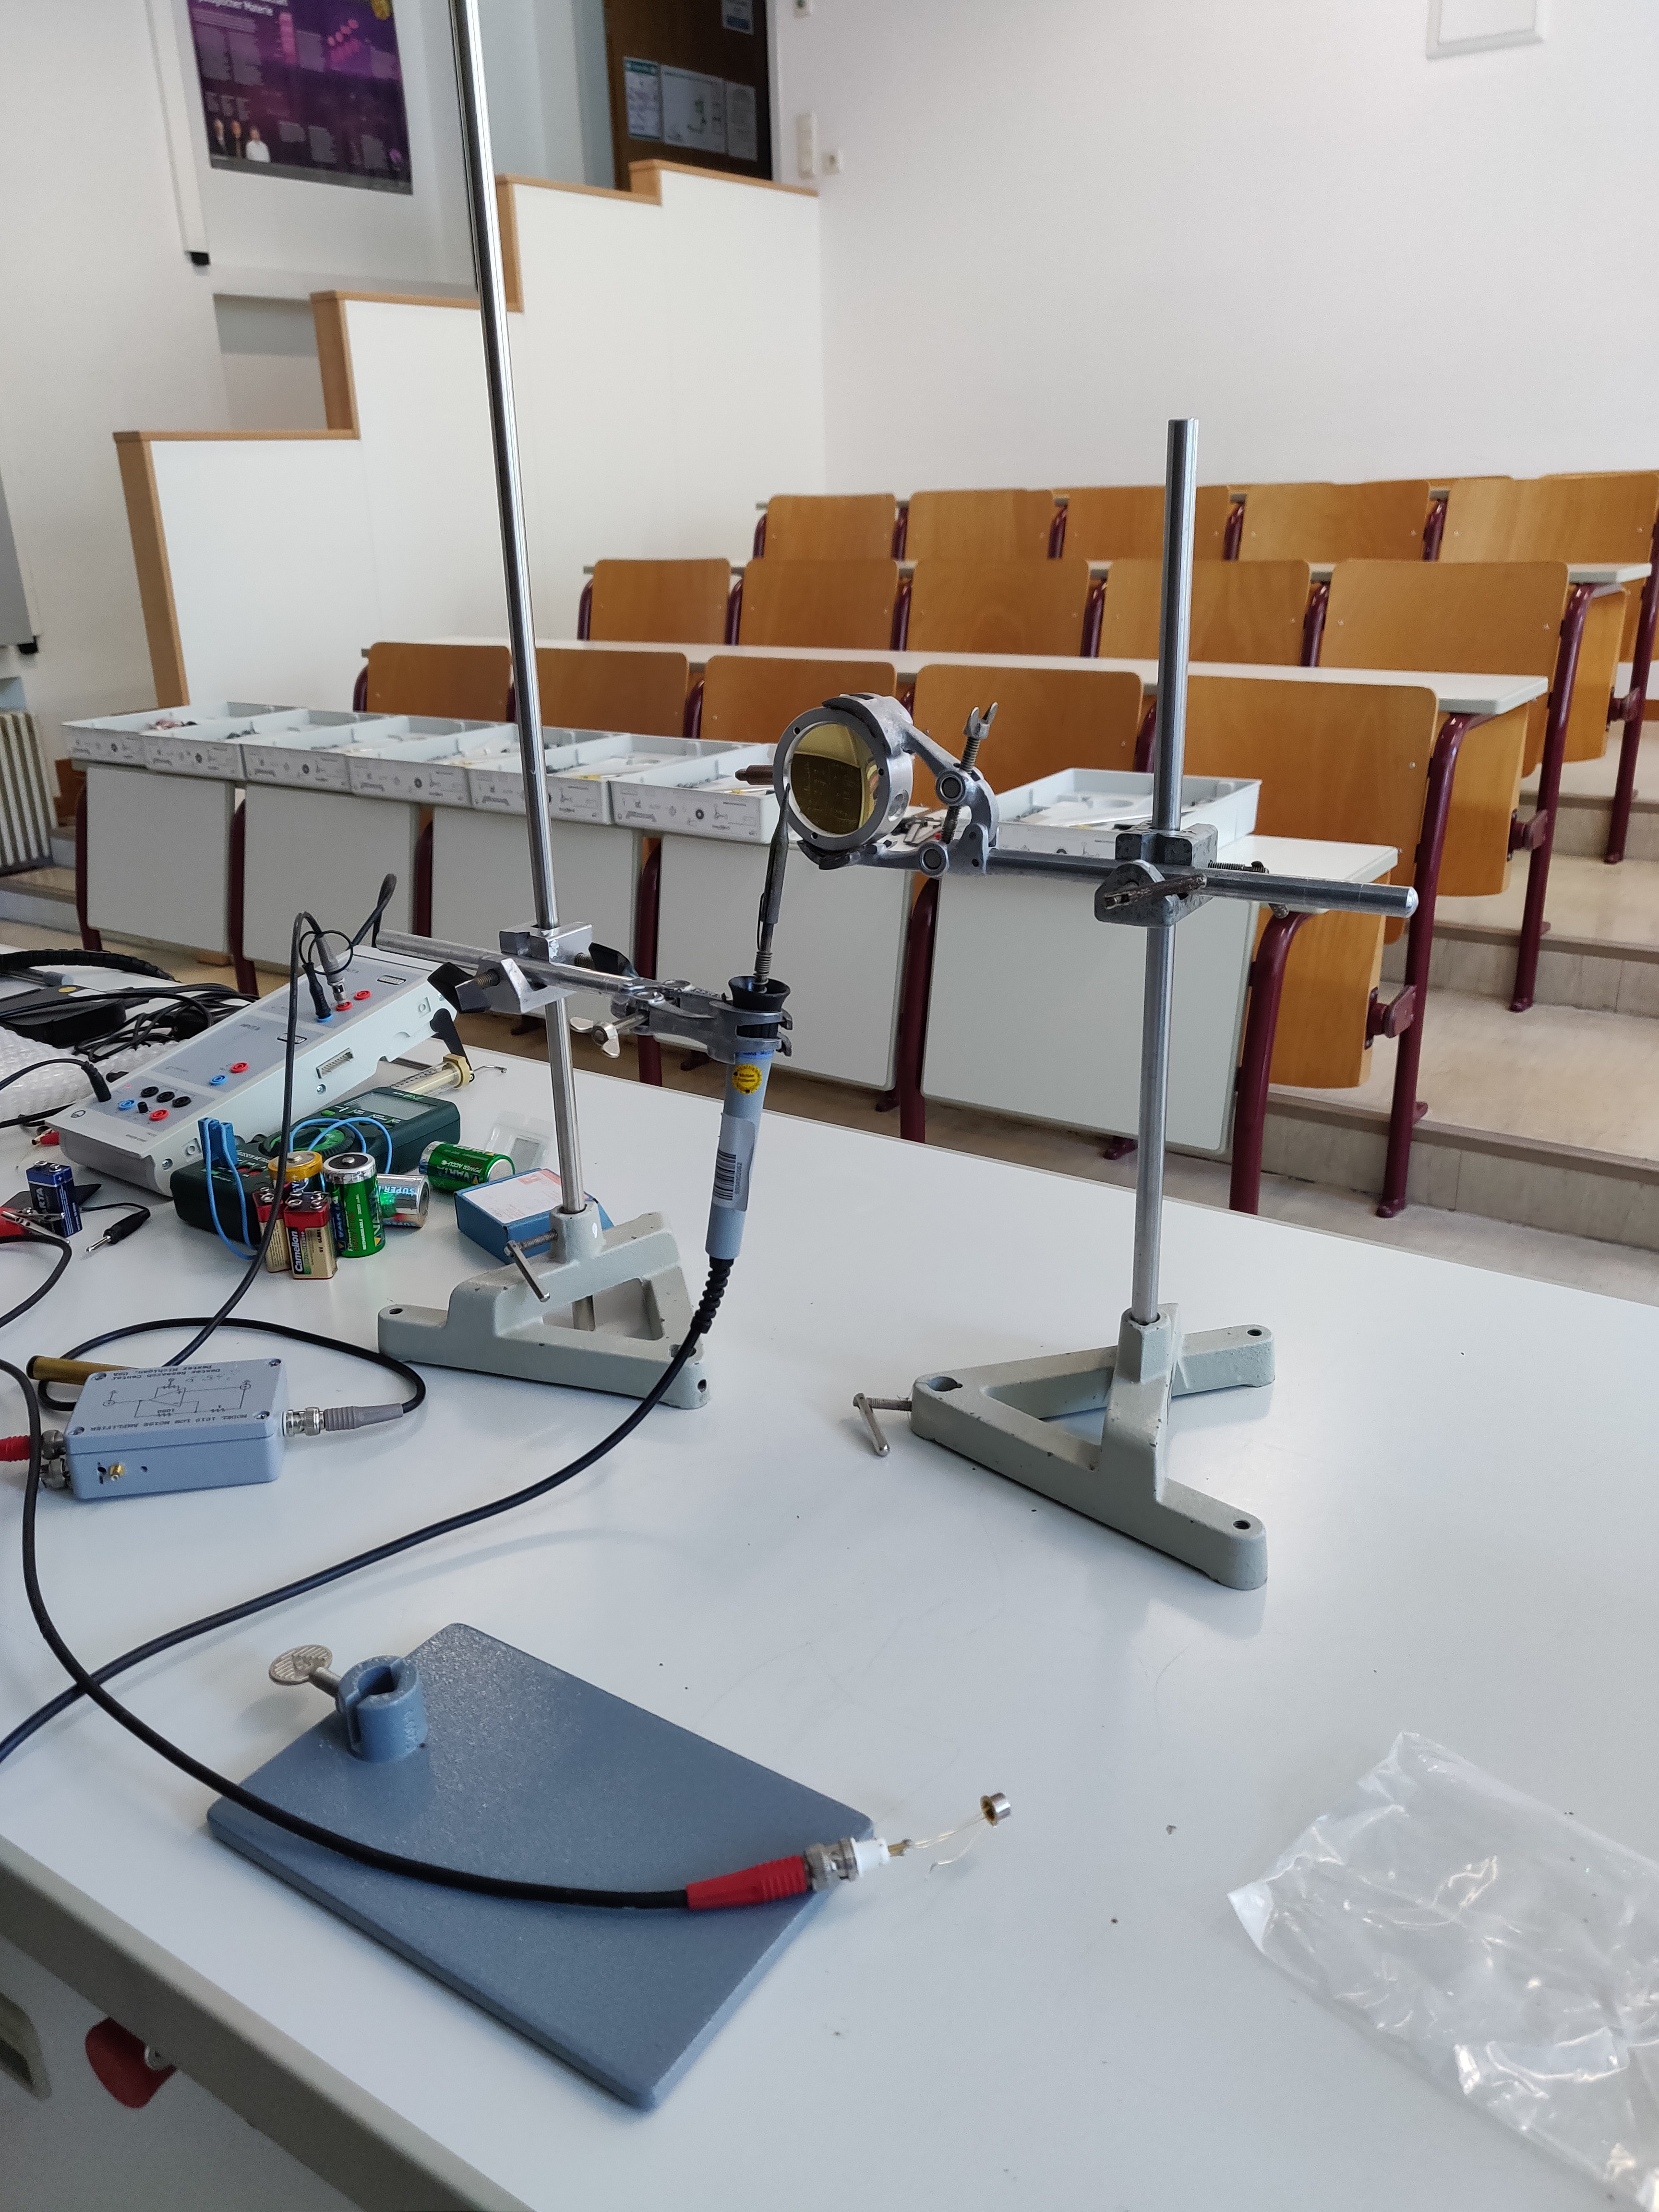
\includegraphics[width=\textwidth]{experiment/13-loetkolben-spiegel.jpg}
        \caption{Lötkolben mit Spiegel}
        \label{fig:loetkolben_mit_spiegel}
    \end{subfigure}
    \begin{subfigure}[b]{0.25\textwidth}
        \includegraphics[width=\textwidth]{experiment/29-leypold-gitter.jpg}
        \caption{Leybold Gitter}
        \label{fig:gitter_600l}
    \end{subfigure}
    \caption{Diverse Komponenten}
\end{figure}

\begin{figure}[ht]
    \centering
    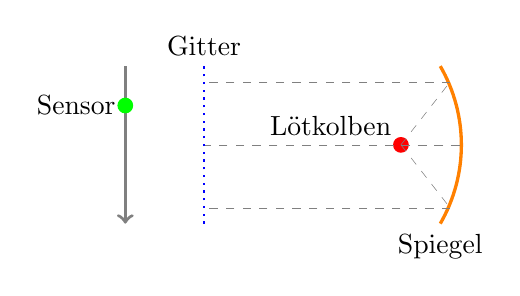
\begin{tikzpicture}
        %\draw[step=1] (-3,-2) grid (4,2);
        
        \draw (3,1)[orange,very thick] arc (30:-30:2cm) node[black,anchor=north] {Spiegel};
        \fill[red] (2.5,0) circle (0.1cm) node[black,anchor=south east] {Lötkolben};
        
        % EM-Strahlungsreflektion
        \draw[gray,dashed,very thin] (2.5,0) -- (3.125,0.8);
        \draw[gray,dashed,very thin] (2.5,0) -- (3.125,-0.8);
        \draw[gray,dashed,very thin] (2.5,0) -- (3.25,0);
        
        \draw[gray,dashed,very thin] (3.125,0.8) -- (0,0.8);
        \draw[gray,dashed,very thin] (3.125,-0.8) -- (0,-0.8);
        \draw[gray,dashed,very thin] (3.25,0) -- (0,0);
        
        \draw[blue,thick,dotted] (0,-1) -- (0,1) node[black,anchor=south] {Gitter};
        
        \draw[very thick,gray,->] (-1,1) -- (-1,-1);
        \fill[green] (-1,0.5) circle (0.1cm) node[black,anchor=east] {Sensor};
    \end{tikzpicture}
    \caption{Aufbau}
    \label{fig:experiment_aufbau}
\end{figure}

\subsubsection{Strahlquelle}
Zunächst benötigen wir eine Infrarot-Strahlquelle, welche die Substanz durchdringt und danach mit einem Detektor gemessen wird. Als Strahlquelle bietet sich ein Lötkolben an (Abb. \ref{fig:loetkolben}), da er bei einer Temperatur von $T = 541K$ Strahlungen in Infrarotbereich abgibt. Das Strahlmaximum lässt sich mit folgender Formel berechnen:

\begin{equation}
    \lambda * T = b
\end{equation}


% λ × T = b
% Lötkolben

\subsubsection{Abbildende Optik}
Um die Strahlung unseres Lötkolbens in eine Richtung zu fokusieren, müssen die nach außen gerichteten Wellen reflektiert werden. Ein Parabelförmiger Spiegel reflektiert die Strahlung so, dass sie in eine Richtung zeigt (Abb. \ref{fig:loetkolben_mit_spiegel}). Der punktförmige Lichtstrahl wird zu einem Parallelstrahl. 

% Spiegel

\subsubsection{Optisches Gitter}
Das Gitter beugt die Strahlung in die verschiedenen Wellenlängen. Hierfür gibt es Gitter verschiedener Linienzahlen pro mm, oder auch Reflexionsgitter, welche sowohl beugen als auch reflektieren (Abb. \ref{fig:gitter_600l}).
Folgende Formel beschreibt die position der Maxima (vielfache von $\lambda$) auf Basis der Strichbreite $b$. 
\[
    k \lambda = b \sin{\alpha}
\]



% 600 Linien / mm
% Leybold
% Reflexionsgitter
